\section{Experimental results}

For our experiments we use a subset of 15 categories of the \emph{Caltech-101} dataset, about 2537 images split between distinct object categories (faces, watches, elephants, motorbikes, etc.)\footnote{\emph{Caltech-101} has been created at the \emph{California Institute of Technology} - http://www.vision.caltech.edu/Image_Datasets/Caltech101/}. Image descriptors are precomputed over the whole dataset and stored on separate files.. All tests were performed on a Mac OSX Notebook with an Intel Core i5, 8GB (running at 2.4 GHz).

Tests have been made on varying of these parameters: train set size, vocabulary size and SIFT descriptor type (\emph{dense, sparse, multi-scale}). Finally, a comparison between \emph{hard} and \emph{soft assignment} is presented. Test set size is always set to 30 (30 images from each category).

In Table \ref{tab:trainsetsize} the classification accuracy on varying training set size (the number shown represent how many images are taken from each category) are shown. As we can see in Table \ref{tab:trainsetsize} the larger the training set size the better the accuracy obtained due the greater number of examples used to create the model.

\begin{table}[h]
\begin{center}
\begin{tabular}{|l|c|c|c|}
\hline
Classifier & 10 & 30 & 50\\
\hline\hline
NN $L_2$ & 38,44 & 53,33 & 52,06\\
NN $\chi^2$ & 59,67 & 67,33 & 67,74\\
SVM Linear & 57,56 & 72,44 & 76,58\\
SVM IK & 72,44 & 79,33 & 83,53\\
SVM $\chi^2$ & 72,44 & 79,56 & 83,27\\
SVM RBF & 57,56 & 71,78 & 72,31 \\
\hline
\end{tabular}
\end{center}
\label{tab:trainsetsize}
\caption{Classification accuracy (\%) on varying training set size}
\end{table}

In Figure \ref{fig:vocabulary} it is shown the classification accuracy variation on growing the vocabulary size. All tests have been made fixing training set size to 30 and using \emph{dense SIFT}. Generally the greater the number of codewords used the greater the accuracy obtained. We attribute this performance boost to the ability of the vocabulary to be more expressive, leading to a more discriminant representation of each image.

\begin{figure}[h]
\begin{center}
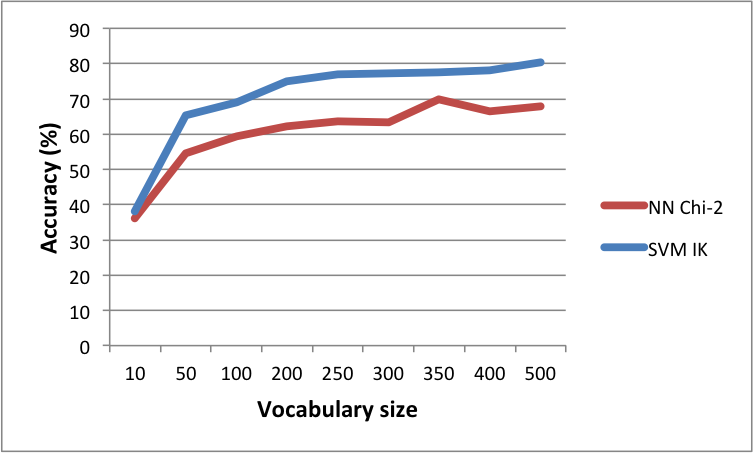
\includegraphics[width=0.45\textwidth]{images/vocabulary.png}
\end{center}
  \caption{Classification accuracy (\%) on growing vocabulary size}
\label{fig:vocabulary}
\end{figure}

In Table \ref{tab:sifttype} it is shown the classification accuracy variation on varying of local features extractor for SIFT descriptor. It is highlighted that dense SIFT reached better accuracy than sparse SIFT due to the greater number of key-points extracted from each images and the spatial homogeneity of key-points distribution. Even better performance is obtained by multi-scale sampling of dense SIFT. 

\begin{table}[h]
\begin{center}
\begin{tabular}{|l|c|c|c|}
\hline
Classifier & \emph{sSIFT} & \emph{dSIFT} & \emph{msdSIFT}\\
\hline\hline
NN $L_2$ & 44 & 49,78 & 52,22\\
NN $\chi^2$ & 57,78 & 68,89 & 68,67\\
SVM Linear & 69,33 & 73,33 & 74,22\\
SVM IK & 77,56 & 81,56 & 81,78\\
SVM $\chi^2$ & 78 & 80 & 82\\
SVM RBF & 71,56 & 71,78 & 71,89 \\
\hline
\end{tabular}
\end{center}
\label{tab:sifttype}
\caption{Classification accuracy (\%) on varying SIFT type}
\end{table}




\begin{figure}[h]
\begin{center}
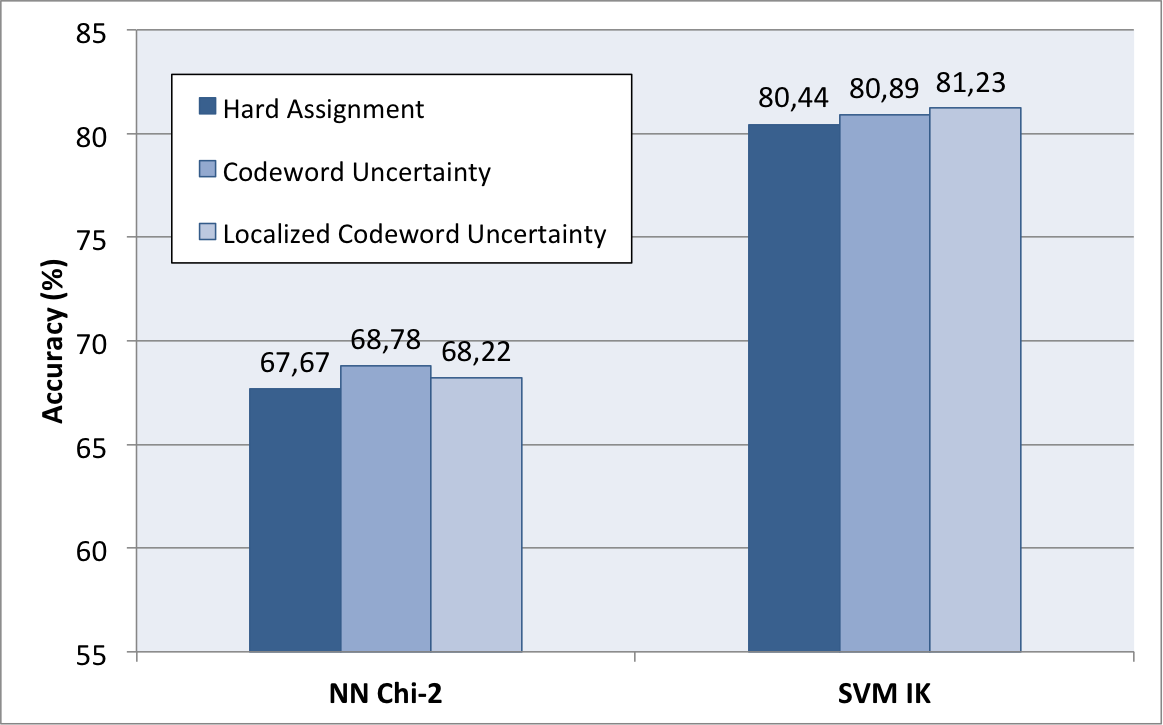
\includegraphics[width=0.45\textwidth]{images/soft-comparison.png}
\end{center}
  \caption{Comparison between hard and soft assignment}
\label{fig:vocabulary}
\end{figure}




